\documentclass[10pt]{article}
\usepackage[utf8]{inputenc}
\usepackage{listings}
\usepackage{float}
\usepackage{graphicx}
\usepackage{fullpage}
\usepackage{caption}
\usepackage{subcaption}
\usepackage{amsmath}
\usepackage{hyperref}
\usepackage{epstopdf}

%\renewcommand{\thesubsection}{\arabic{subsection}}
\renewcommand{\thesubsubsection}{\alph{subsubsection}}

\title{Signals and Systems Lab 1}
\author{Maikel Withagen (s1867733) \and Steven Bosch (s1861948)}
\date{\today}
\lstset{
frame=single,
numbers=left,
breaklines=true,
language=Matlab,
basicstyle=\footnotesize,
title=\lstname,
showstringspaces=false
}

\renewcommand{\thesubsection}{\small(\alph{subsection})}
\begin{document}
\maketitle

\section{Summing Sinusoids}
\subsection{}
Our implementation of the function gensinusoid is given in section A(a) of the appendix.

\subsection{}
Using the function given in the previous section we get the graph given in figure \ref{fig1b}. The amount of samples that corresponds to one oscillation is $f_s/f=8000/400=20$.
\begin{figure}[H]
  \centering
  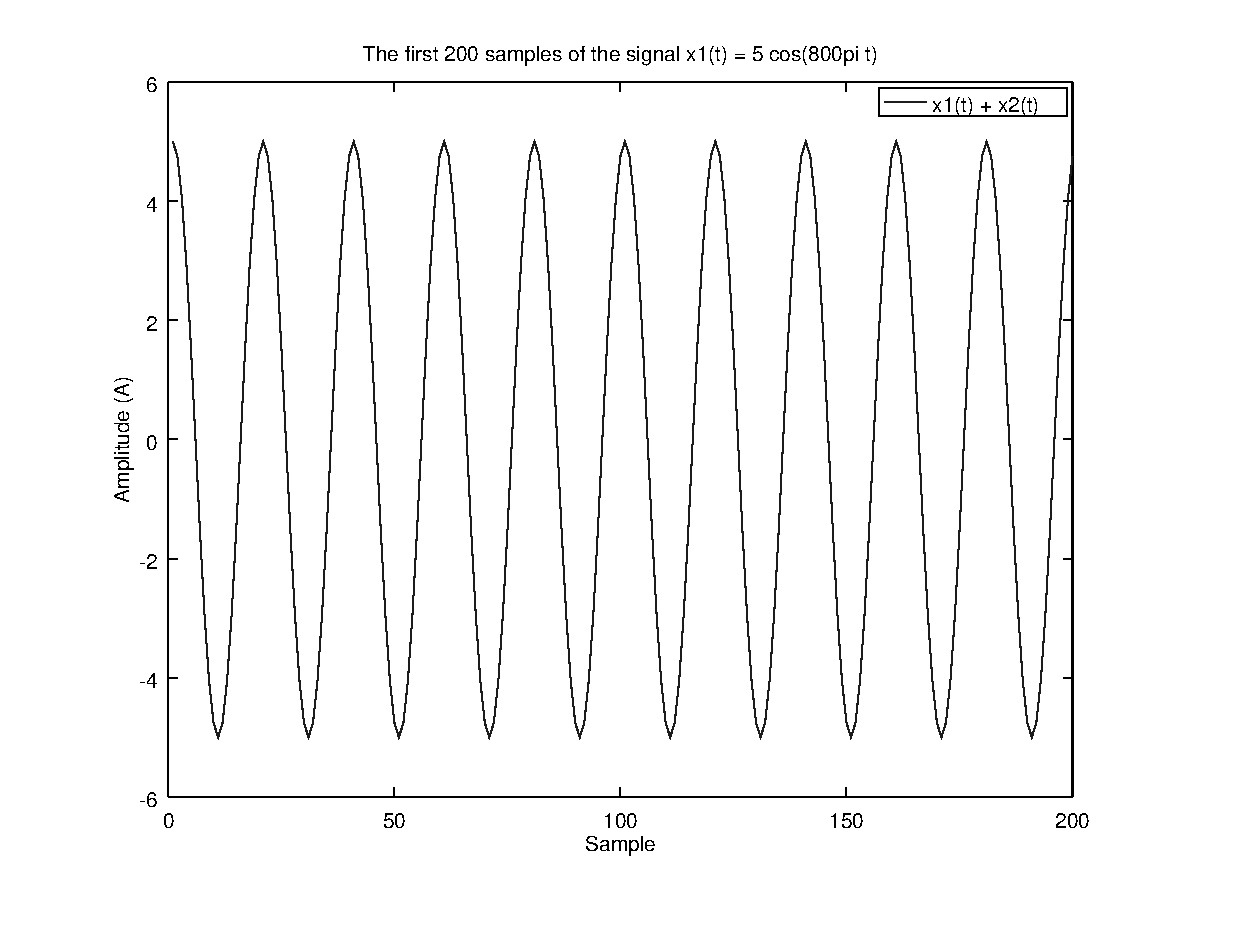
\includegraphics[width=.8\columnwidth]{plot1A.eps}
  \caption{The first 200 samples of the signal $x1(t) = 5cos(800\pi t)$}
  \label{fig1b}
\end{figure}

\subsection{}
Our implementation of the function sumsinusoid is given in section A(b) of the appendix.

\subsection{}
The shift of $0.013125s$ translates to a period of $\omega * t = 800\pi*0.013125 = 10.5\pi$. Now we have the following formulas:
\begin{equation}
    x1(t) = 5 cos(800\pi t)
\end{equation}
\begin{equation}
    x2(t) = 5 cos(800\pi t + 10.5\:pi)
\end{equation}
We can generate x1(t)+x2(t) by plotting the sum of the separate generated functions given by the function gensinusoid, resulting in figure \ref{fig2d1}.\\
\begin{figure}[H]
  \centering
  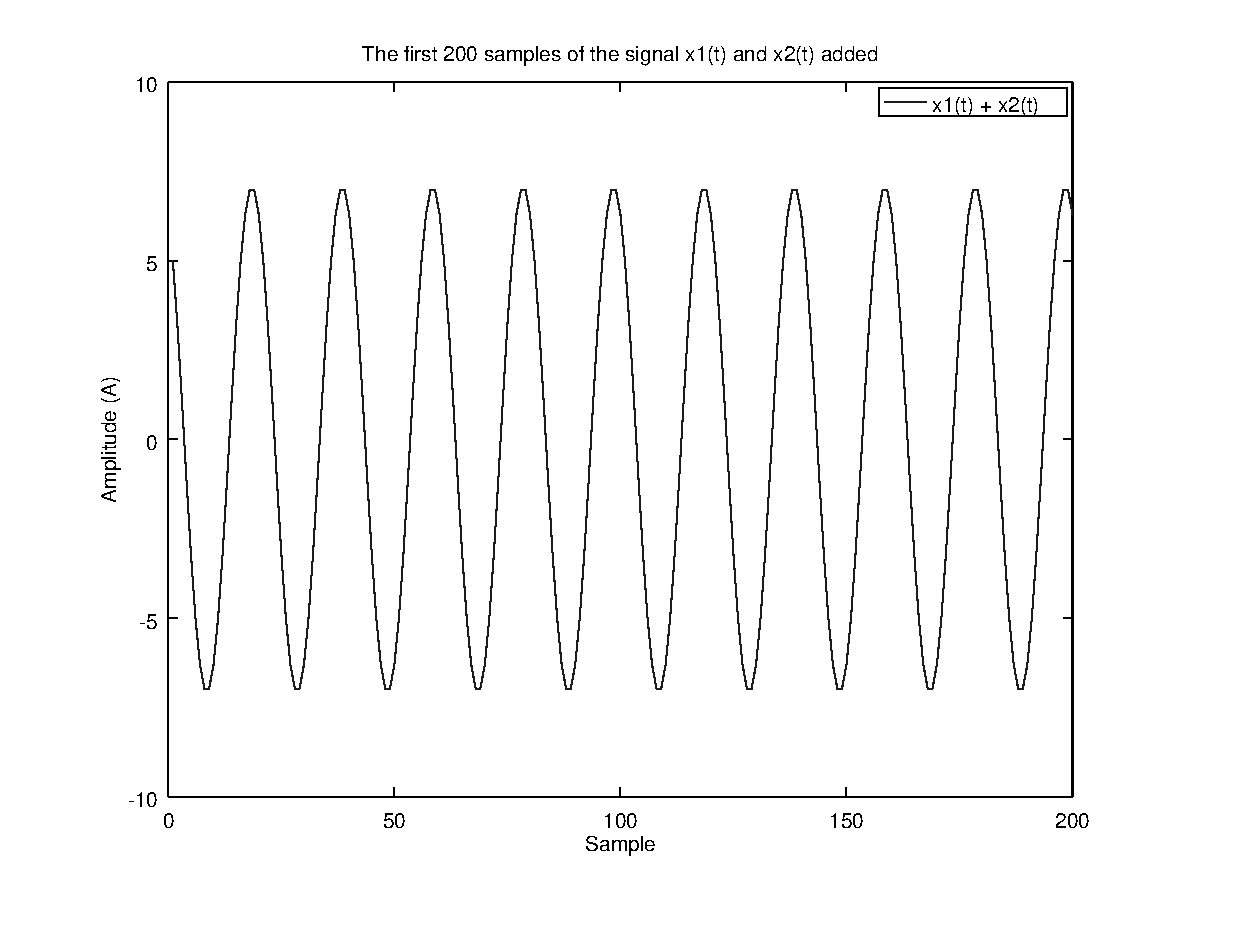
\includegraphics[width=\columnwidth]{plot4A.eps}\\
  \caption{The first 200 samples of the signal x1(t) and x2(t) added.}
  \label{fig2d1}
\end{figure}
Using the sumsinusoid function we can calculate the values for y(t):
$[A, f, phi] = 7.07107,400.00000,0.78540$, giving us\
\begin{equation}
    y(t) = 7.07107 cos(400*2*\pi t + 0.78540)
\end{equation}
The plot with both lines, given in figure \ref{fig2d2}, shows a perfect overlap, so we can conclude that our answer for y(t) is the same as the sum of the two functions. See section A(c) in the appendix for the script that executes the described process.

\begin{figure}[H]
  \centering
  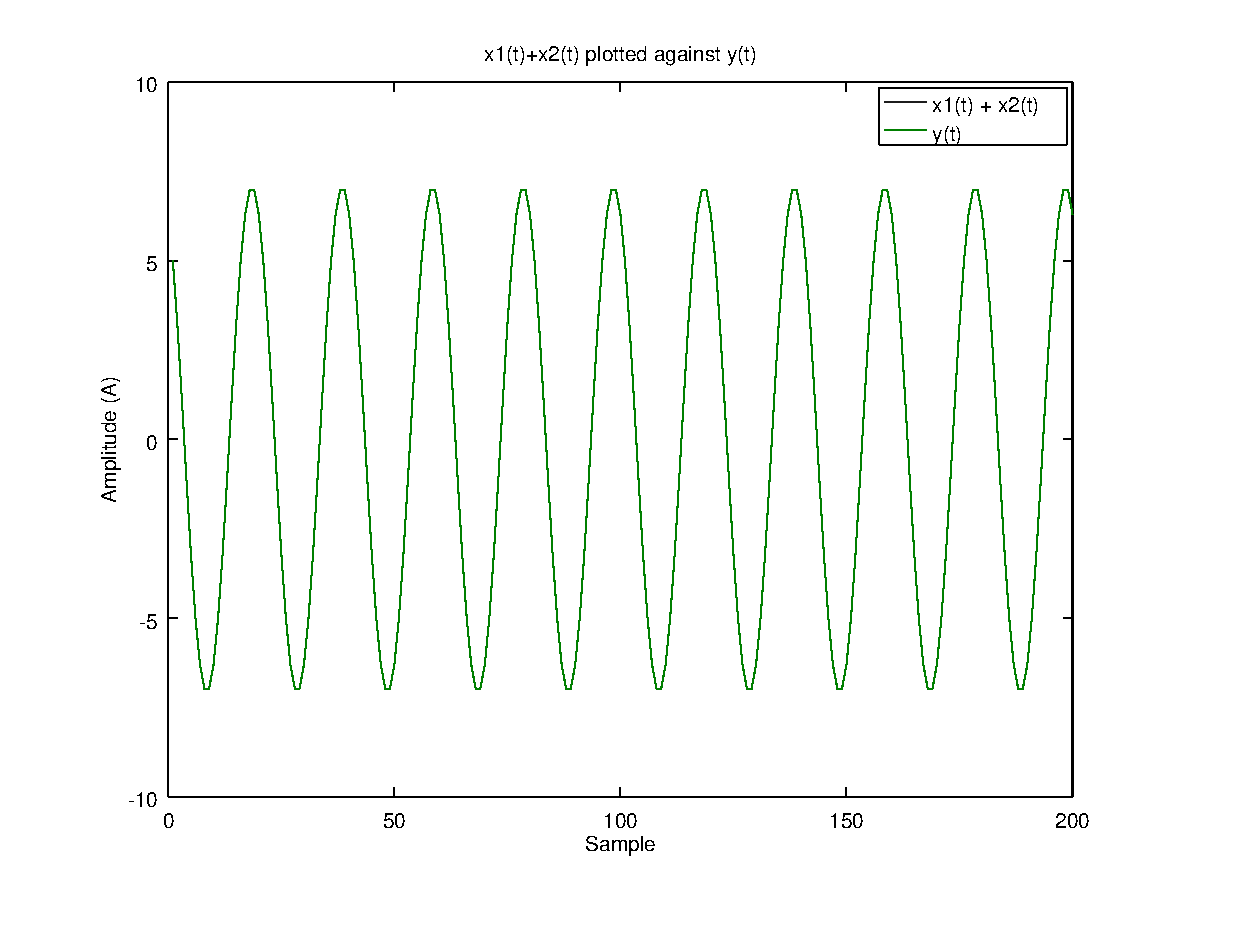
\includegraphics[width=\columnwidth]{plot4B.eps}
  \caption{x1(t)+x2(t) and y plotted in the same figure.}
  \label{fig2d2}
\end{figure}

\subsection{}
\begin{figure}[H]
  \centering
  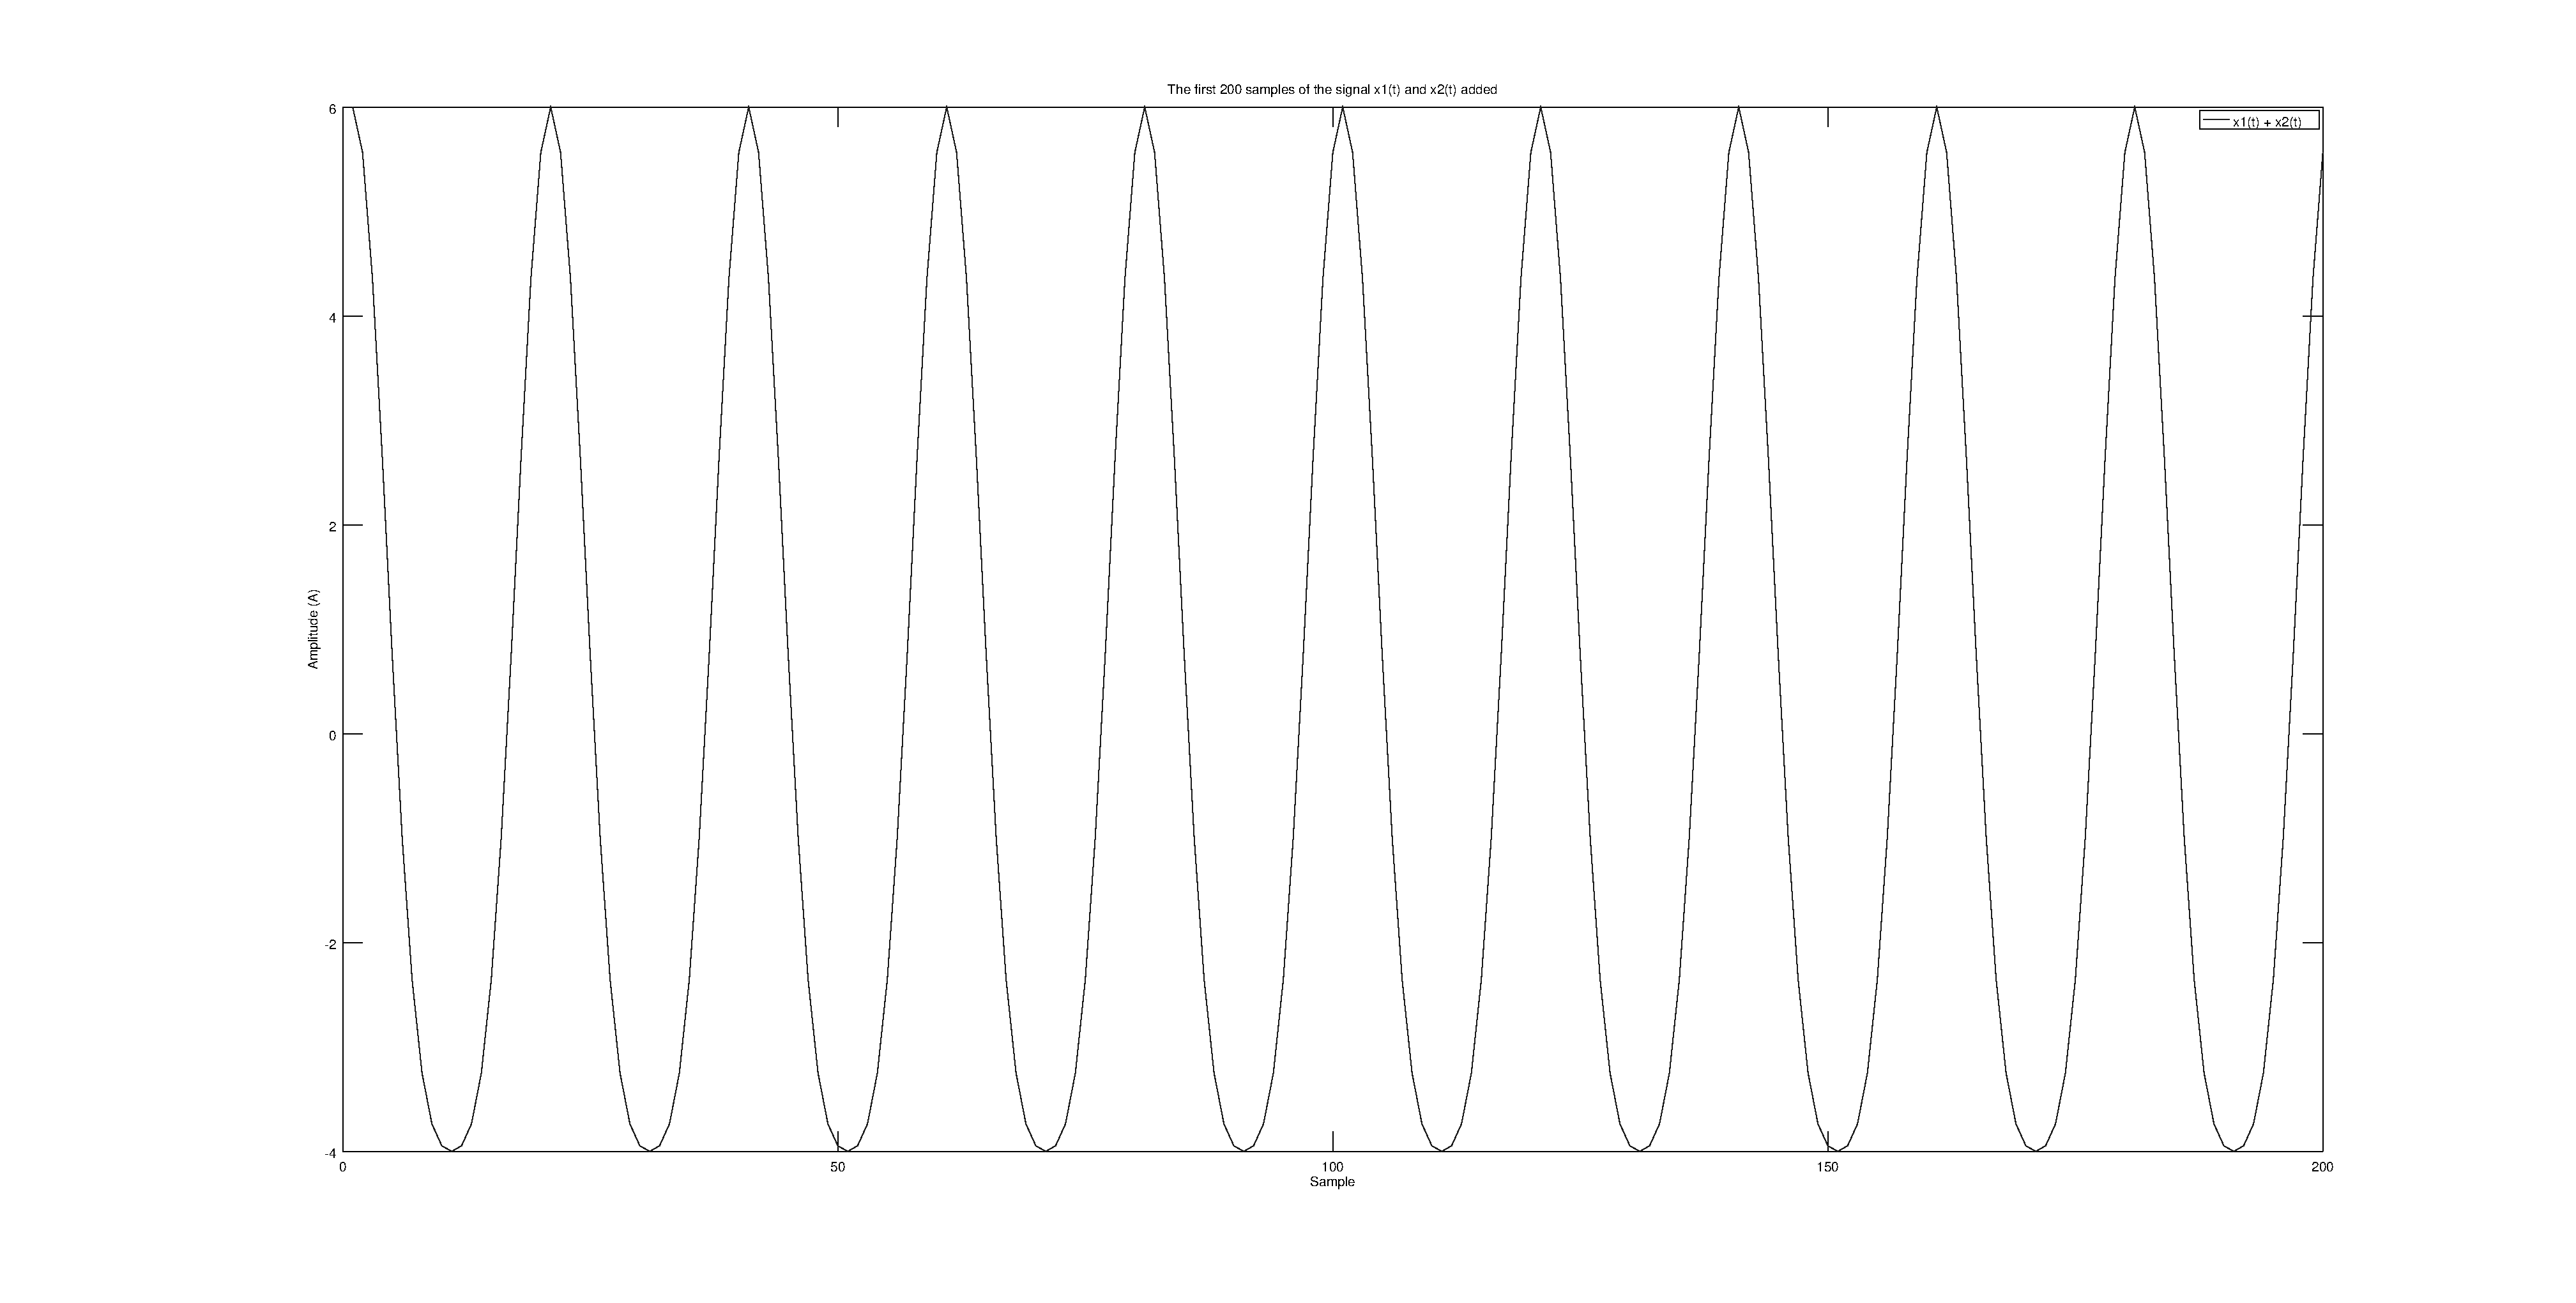
\includegraphics[width=\columnwidth]{plot1E.eps}\\
  \caption{}
  \label{fig1e}
\end{figure}

\newpage
\section*{Appendix}
\appendix
\section{Summing Sinosoids}
\subsection{gensinusoid}
\lstinputlisting{../code/gensinusoid.m}
\subsection{sumsinusoid}
\lstinputlisting{../code/sumsinusoid.m}
\subsection{Verification script 1d}
\lstinputlisting{../code/1d.m}

\end{document}
